\subsection{UML-проектирование}

Первоначальной стадией разработки программного продукта является стадия проектирования.
В качестве проектного {\it CASE}-средства был выдран продукт {\it Visual Paradigm}.
С помощью его было составлена диаграмма классов (см. рис. ~\ref{ris:UML}), на основе которой был сгенерирован начальный код программного решения.

\begin{figure}[h]
\center{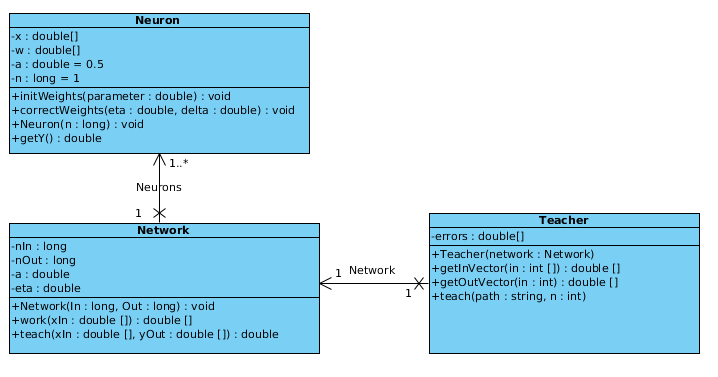
\includegraphics[width=1\linewidth]{uml}}
\caption{Диаграмма классов программного решения}
\label{ris:UML}
\end{figure}